\chapter{Background}
To better understand this thesis work, a brief excursus of the existing literature about the main concepts the project relies on is presented. The aim is to provide some basic knowledge of the topics to understand what is considered state-of-the-art and to introduce some of the technologies exploited to develop the project.

\section{Multi-Agent Systems}
Multi-Agent Systems are considered a promising engineering style for developing adaptive software systems able to handle the continuous increase in their complexity.
Moreover, they allow the design and implementation of software systems using the same ideas and concepts that are the very founding of human societies and habits.

In this section, a brief overview of the main concepts and characteristics of MAS is provided, as well as the main approaches to their design.

\subsection{What is an Agent?}
The concept of a software agent can be traced back to the early days of research into Distributed AI in the 1970s when Carl Hewitt proposed the concurrent Actor model.
In his paper, he introduced the concept of a self-contained, interactive, and concurrently-executing object which he termed ``actor''.
The latter is a computational agent with a mail address and behavior. Actors can communicate by message-passing and carry out their actions concurrently.~\cite{hewitt1977viewing}

The term ``agent'' quickly spread to heterogeneous research fields; therefore, there is no commonly agreed definition for it.
However, a generally accepted description of what an agent is is the following by Wooldridge~\cite{490039}:
\begin{quote}
    \textit{An agent is a self-contained program capable of controlling its own decision-making and acting, based on its perception of its environment, in pursuit of one or more objectives.}
\end{quote}
To sum up, a set of features that an agent should possess can be identified:
\begin{itemize}
    \item \textbf{Autonomy}: agents should be able to perform most of their tasks without the direct intervention of humans or other agents, and they should encapsulate control over their actions and internal state
    \item \textbf{Social ability}: agents should be able to interact with each other and possibly humans to complete their tasks.
    \item \textbf{Responsiveness} (situatedness): agents should perceive their environment and respond to changes in it.
    \item \textbf{Proactiveness}: agents should exhibit opportunistic, goal-directed behavior and take the initiative when appropriate.
\end{itemize}

During the first years, the research concentrated on interaction and communication among agents, decomposition and distribution of tasks, and coordination and cooperation.
The goal was to specify, analyze, design, and integrate systems containing multiple collaborative agents.

\subsection{From the Individual to the Collective}
Multi-Agent Systems have been studied as a per se field since the 1980s and gained widespread recognition in the 1990s.
Since then, international interest in the topic has grown enormously as agents are considered an appropriate paradigm to exploit the possibilities presented by massive open distributed systems.
Moreover, MAS seem to be a natural metaphor for understanding and building a wide range of what might be called \textit{artificial social systems}.~\cite{wooldridge2009introduction}

According to the \textit{Alan Turing Institute}~\cite{turing}
\begin{quote}
    \textit{A Multi-Agent System consists of multiple decision-making agents which interact in a shared environment to achieve common or conflicting goals.}
\end{quote}

\begin{figure}
    \centering
    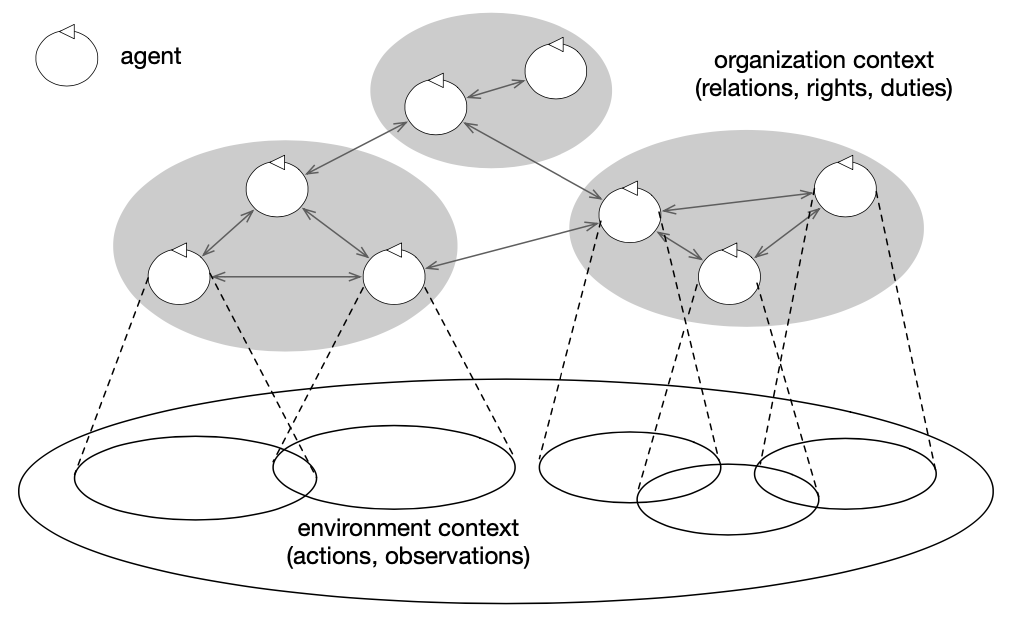
\includegraphics[width=0.9\linewidth]{images/multi-agent-systems.png}
    \caption{A representation of Multi-Agent Systems.~\cite{jennings2000agent}}
    \label{fig:multi-agent-systems}
\end{figure}
Therefore, as it can also be noticed in \cref{fig:multi-agent-systems}, MAS are composed of an environment and agents existing within it that are bonded by relations.

\section{Multi-Agent Oriented Programming}
In principle, there is no constraint on the programming technologies that can be used to implement MAS.
However, the risk is to have an agent-centered interpretation of the system in which the environment and/or the organization contexts are represented and managed in the mind of the agents.
Therefore, the adoption of programming languages and paradigms that directly support first-class abstractions for these contexts highly simplifies the task of designing and implementing MAS and makes it possible to keep the level of abstraction coherent from design time to development time and finally also at runtime.

\textit{Multi-Agent Oriented Programming} (MAOP) is an approach to programming MAS that promotes the use of first-class programming abstractions that concern three main dimensions that characterize these systems:~\cite{boissier2020multi}
\begin{itemize}
    \item \textbf{Agent dimension}: it concerns the concepts and programming abstractions for the definition of the agents that participate in the system.
    Specifically, it allows the definition of software entities with their logical thread of control, which can autonomously and proactively achieve their goals, and interact with the environment, other agents, and the organization that regulates the system.
    \item \textbf{Environment dimension}: it offers concepts and abstractions to define the distributed resources and connections to the world shared among the agents.
    Thus, the environment abstraction is what makes the agents situated and provides them with tools that help them achieve their goals.
    \item \textbf{Organization dimension}: it collects all the concepts regarding the definition of relations, shared tasks, and policies among agents (inter)acting in a shared environment.
    In open systems, the organization is fundamental for coordination and regulation among agents.
\end{itemize}

Since agents have already been discussed, the following sections provide a description of the latter two dimensions, with a particular focus on the one regarding the organization, as it is the core of this thesis work.

\subsection{Environment in Multi-Agent Systems}
The environment in MAS plays a dual role~\cite{weyns2007environment}:
\begin{itemize}
    \item \textit{The ``external world''}:
    agents become aware of the context they are immersed in and its dynamics by perceiving the environment through sensors.
    Moreover, they pursue their goals through actions performed by actuators that aim at modifying the environment, eventually reaching the latter's desired state.
    \item \textit{A medium for coordination}:
    agents exploit the environment to share information and coordinate their behavior.
    Each agent follows simple behavioral rules, resulting in a collective behavior that is more complex than the sum of the individual behavior; this pattern resembles stigmergic systems in which agents coordinate their behavior through the manipulation of marks.
\end{itemize}
The environment not only enables the agents to interact with the deployment context, which they can access through sensors and actuators, but also provides them with external resources that they can exploit to achieve their goal.

The \textit{Agents \& Artifacts} (A\&A) conceptual framework~\cite{ricci2007artifacts} argues that, just like in human society, MAS environments should contain different kinds of objects, tools, and artifacts in general that agents can use to support their activities.
This vision also constitutes a revolution from an engineering perspective as it encourages system designers to model the environment as a set of \textit{artifacts}, each of which encapsulates its intended purpose and exposes its observable state.
Moreover, the A\&A meta-model provides an effective abstraction level that shields low-level details of the deployment context, so that designers can focus on the agents' behavior.

\subsection{Organization in Multi-Agent Systems}
An agent organization can be defined as a social entity composed of a specific number of agents that accomplish several common tasks or goals and that are structured following some specific topology and communication interrelationships to achieve the main aim of the organization.
All MAS possess some form of organization, although it may be implicit and informal.

\subsubsection{Approaches to Organization in MAS}
There are two approaches to MAS engineering.~\cite{Ahmed_Abbas_2015}
The first one regards \textit{agent-centered} MAS, in which the focus is given to individual agents.
According to this viewpoint, the designer should concern about the local behavior of the agents and their interactions without worrying about the global structure and goal of the system as the latter should emerge as a result of the lower-level individual interactions in a bottom-up fashion.
The key issues of this approach are unpredictability and uncertainty since it could lead to undesirable emergent behaviors.
As Weyns~\cite{weyns2010organizations} stated, giving the responsibility of system organization implicitly to individual agents is highly complex and not suitable for real-world large-scale scenarios.

The second approach is \textit{organization-centered} MAS, in which the structure of the system is given greater attention.
The developer designs the entire organization and coordination patterns on the one hand, and the agents' local behavior on the other.
This can be seen as a top-down approach as the organization abstractions impose constraints on the agents and regulate their interactions, simplifying the design of complex and scalable systems and allowing more accurate modeling of the problems being tackled.

\subsubsection{Organizational Paradigms}
Although no two organizational instances are likely to be identical, there are identifiable classes of organizations, that emerged from research and real-world applications, which share common characteristics.
These classes are called \textit{organizational paradigms} and cover particularly common, useful, or interesting structures that can be described in some general form.
Here is provided a brief overview of the most common paradigms~\cite{horling_lesser_2004}:
\begin{itemize}
    \item \textbf{Hierarchies}: agents are conceptually arranged in a tree-like structure, where agents higher in the tree have a more global view than those below them.
    Interactions only take place between connected entities; data produced by lower-level agents in a hierarchy typically travels upwards to provide a broader view, while control flows downwards as the higher-level agents provide directions to those below.
    \item \textbf{Holarchies}: agents are organized in holons.
    The term \textit{holon} comes from the Greek words \textit{holos}, meaning ``whole'', and \textit{on}, meaning ``part''. Therefore, a holon is a self-contained entity that can be considered both as a part of a larger entity and as a whole in itself, and that has a character derived but distinct from the entities that make it up and at the same time it contributes to the properties of a greater whole.
    \item \textbf{Coalitions}: they are formed by agents that share a common goal and that are willing to cooperate to achieve it and are generally short-lived as they are formed with a purpose in mind and dissolved when that need no longer exists.
    Although there may be a distinguished ``leading agent'', within a coalition the structure is typically flat.
    However, since once formed coalitions may be treated as a single entity, it is possible to form a hierarchical structure by nesting coalitions.
    \item \textbf{Teams}: they consist of several cooperative agents that agreed to work together towards a common goal.
    Unlike coalitions, teams attempt to maximize the performance of the group as a whole, rather than the performance of individual agents.
    This is usually achieved by assigning roles to the agents, which become responsible for specific tasks, and by providing the agents with representations of the shared goals, knowledge and plans.
    \item \textbf{Congregations}: although similar to the latter two structures, they differentiate because are assumed to be long-lived and are not necessarily formed with a specific goal in mind.
    Indeed, congregations are formed among agents with similar o complementary characteristics to facilitate the process of finding partners for collaborations.
    \item \textbf{Societies}: they are open systems where agents of different kinds may come and go at will while the society persists, acting as an environment through which the participants meet and interact.
    Societies impose on agents a set of constraints which are known as \textit{social laws}, \textit{norms} or \textit{conventions}.
    These represent rules by which agents must act and provide a level of consistency in behavior that facilitates the coexistence of possibly heterogeneous agents.
    \item \textbf{Federations}: they are groups of agents which have ceded some amount of autonomy to a single delegate who represents the group.
    The members of the group interact only with the delegate, who accepts skills and needs descriptions from them, which are then used to match with requests from delegates representing other groups.
    \item \textbf{Markets}: buying agents may request or place bids for a common set of items, such as shared resources, tasks, services, or goods, or even supply items to the markets to be sold.
    On the other hand, sellers are responsible for processing bids and determining the winner.
    \item \textbf{Matrix}: they can be seen as a relaxation of the one-agent, one-manager restriction in hierarchical organizations, that permit many managers to influence the activities of an agent.
\end{itemize}

\begin{figure}
    \begin{subfigure}[h]{0.3\linewidth}
        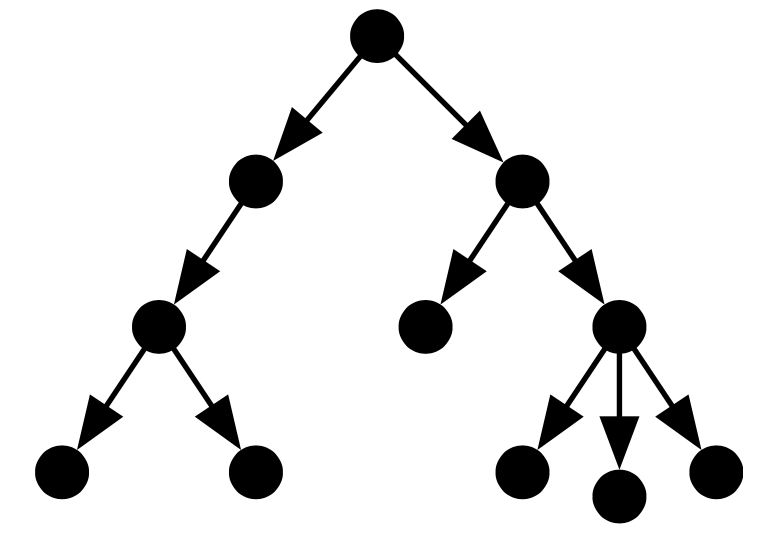
\includegraphics[width=\textwidth]{images/orgs/org-hierarchy.png}
        \caption{Hierarchiy}
        \label{fig:hierarchy}
    \end{subfigure}
    \begin{subfigure}[h]{0.3\linewidth}
        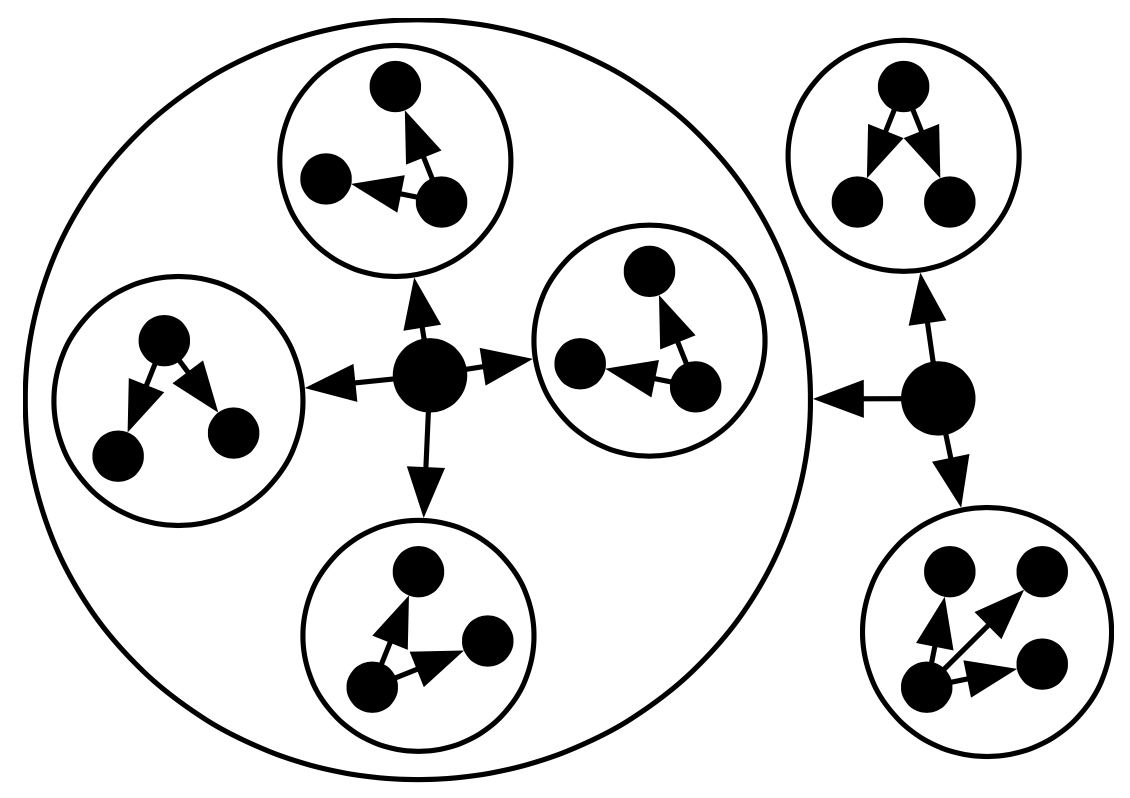
\includegraphics[width=\textwidth]{images/orgs/org-holarchy.png}
        \caption{Holarchy}
        \label{fig:holarchy}
    \end{subfigure}
    \begin{subfigure}[h]{0.3\linewidth}
        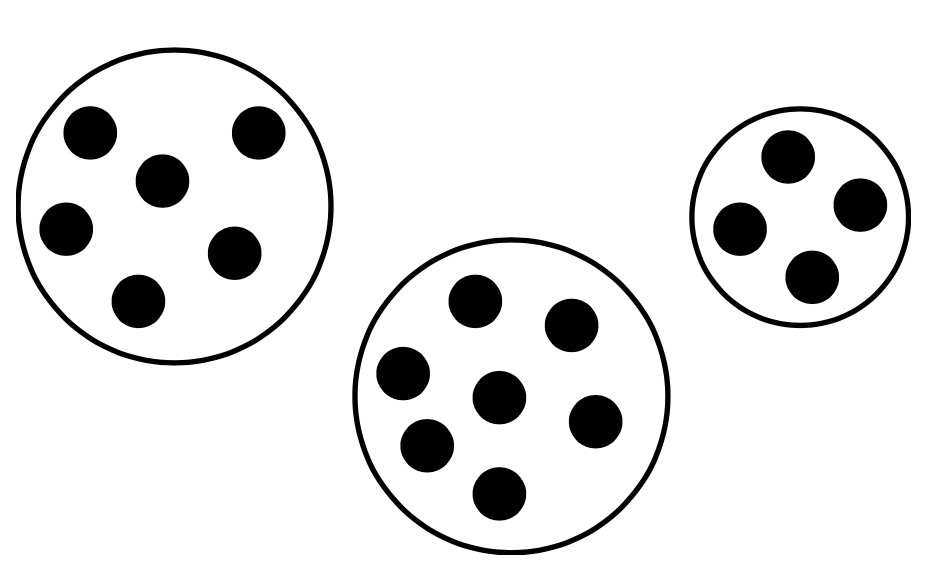
\includegraphics[width=\textwidth]{images/orgs/org-coalitions.png}
        \caption{Coalitions}
        \label{fig:coalitions}
    \end{subfigure}
    \begin{subfigure}[h]{0.3\linewidth}
        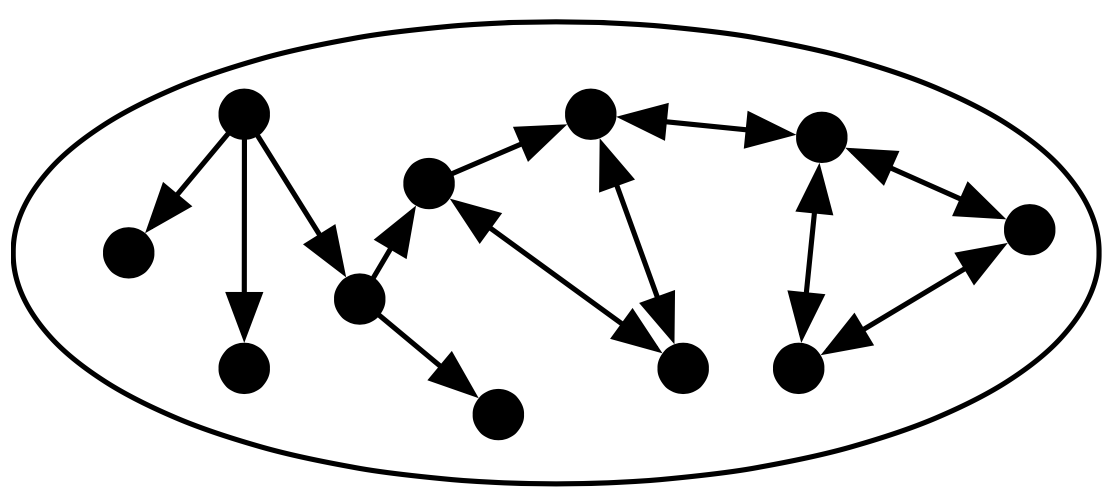
\includegraphics[width=\textwidth]{images/orgs/org-teams.png}
        \caption{Team}
        \label{fig:teams}
    \end{subfigure}
    \begin{subfigure}[h]{0.25\linewidth}
        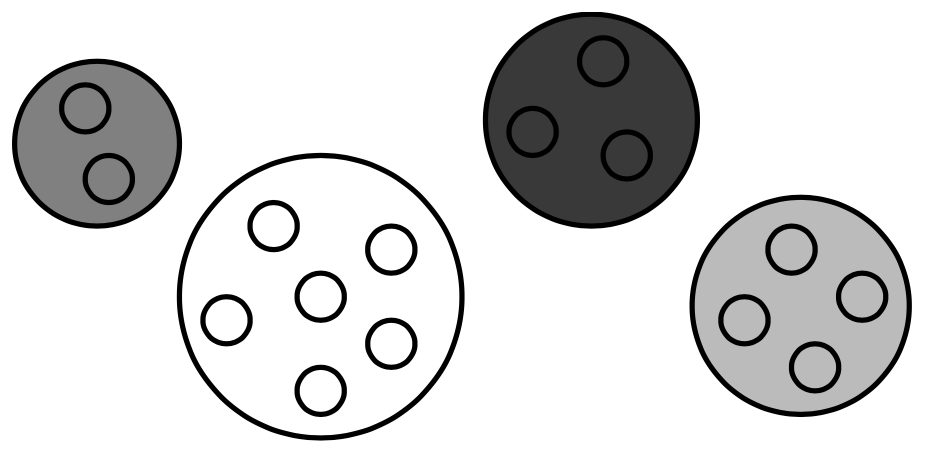
\includegraphics[width=\textwidth]{images/orgs/org-congregations.png}
        \caption{Congregations}
        \label{fig:congregations}
    \end{subfigure}
    \begin{subfigure}[h]{0.3\linewidth}
        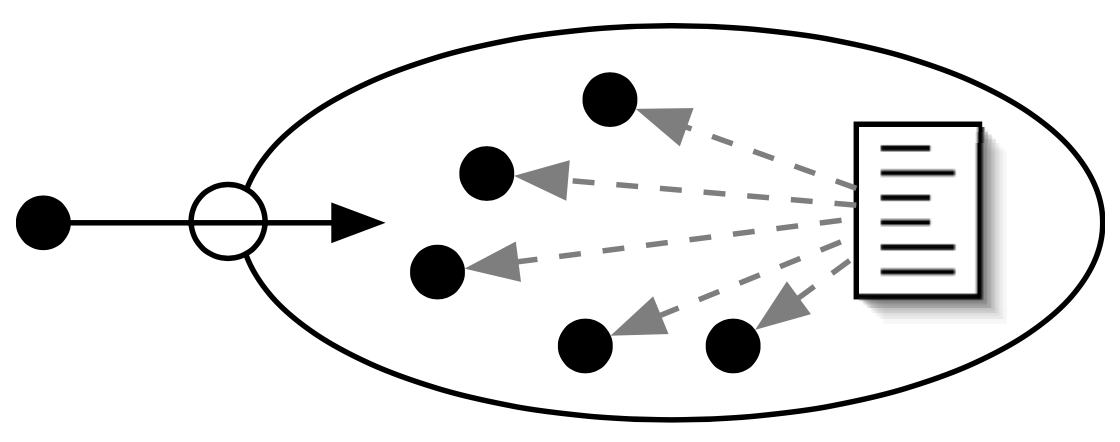
\includegraphics[width=\textwidth]{images/orgs/org-societies.png}
        \caption{Society}
        \label{fig:societies}
    \end{subfigure}
    \begin{subfigure}[h]{0.3\linewidth}
        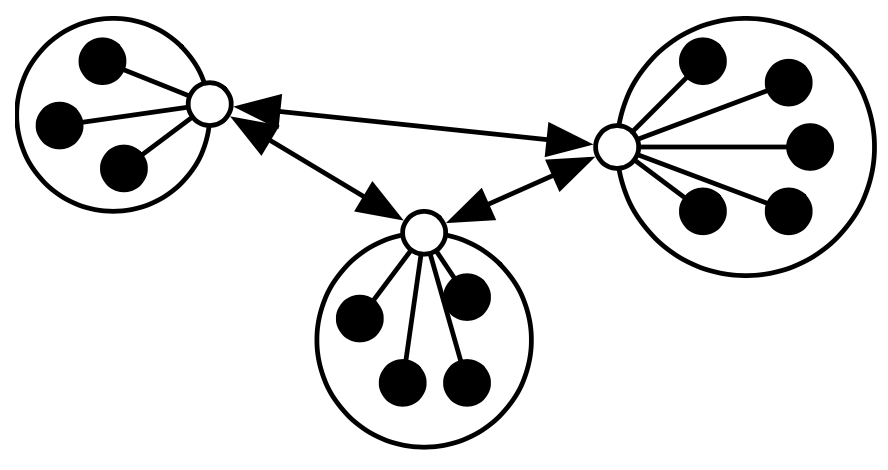
\includegraphics[width=\textwidth]{images/orgs/org-federations.png}
        \caption{Federations}
        \label{fig:federations}
    \end{subfigure}
    \begin{subfigure}[h]{0.3\linewidth}
        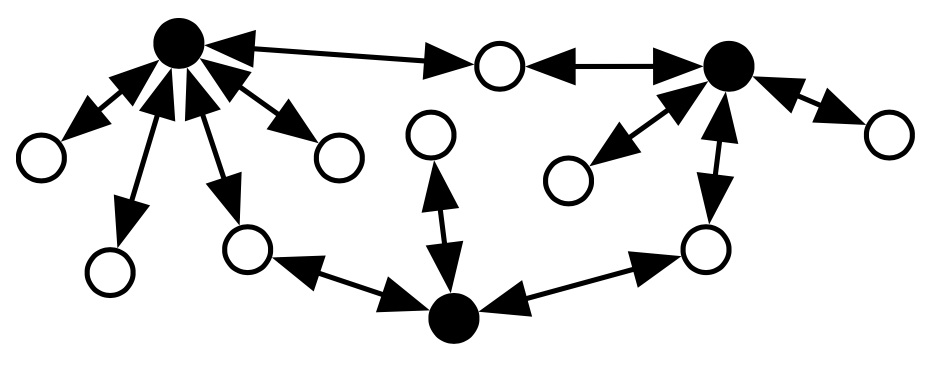
\includegraphics[width=\textwidth]{images/orgs/org-markets.png}
        \caption{Markets}
        \label{fig:markets}
    \end{subfigure}
    \begin{subfigure}[h]{0.3\linewidth}
        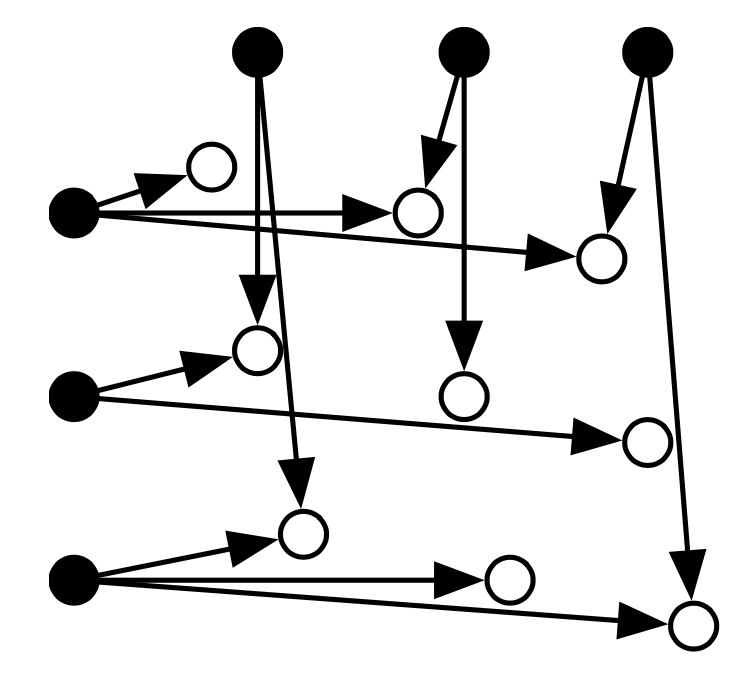
\includegraphics[width=\textwidth]{images/orgs/org-matrix.png}
        \caption{Matrix}
        \label{fig:matrix}
    \end{subfigure}
    \caption{Visual representation of the organizational paradigms.}
    \label{fig:organizational-paradigms}
\end{figure}

All of the above structures come with their benefits and drawbacks, which are briefly summarized in~\cref{table:orgs-advantages-disadvantages} and it is generally agreed that there is no single type of organization that is suitable for all situations.
Indeed, sometimes two or more organizational paradigms may be combined to form a compound organization, exploiting features of each of the component organizations.


\begin{table}[h]
    \centering
    \begin{tabular}{ | l p{0.4\linewidth} p{0.4\linewidth} | }
        \hline
        \textbf{Paradigm} & \textbf{Benefits} & \textbf{Drawbacks} \\\hline\hline
        Hierarchy & Maps to many common domains; handles scale well & Potentially brittle; can lead to bottlenecks \\\hline
        Holarchy & Exploit autonomy of functional units & Must organize holons, lack of predictable performance. \\\hline
        Coalition & Exploit strength in number & Individual goals are preferred to common goals \\\hline
        Team & Address larger problems; task-centric & Increased communication \\\hline
        Congregation & Facilitates agents discovery & Sets may be overly restrictive \\\hline
        Society & Public services; well-defined conventions & Potentially complex; agents may require society-related capabilities \\\hline
        Federation & Matchmaking, brokering, and translation services facilitate dynamic agent pool & Intermediaries become bottlenecks \\\hline
        Market & Good at allocation, increased utility through centralization, increased fairness through bidding & Potential for malicious behavior; decisions complexity can be high \\\hline
        Matrix & Resource sharing; multiple influenced agents & Potential conflicts \\\hline
    \end{tabular}
\caption{Benefits and drawbacks of the organizational paradigms, adopted from~\cite{Ahmed_Abbas_2015}.}
\label{table:orgs-advantages-disadvantages}
\end{table}

\subsection{The JaCaMo Platform}
Regarding the engineering and implementation of MAS, one of the reference technologies is the JaCaMo platform~\cite{Boissier2016}, which supports practical programming based on the first-class abstractions introduced before to develop organized agents situated in a shared environment.
JaCaMo is built on top of three other existing platforms:
\begin{itemize}
    \item \jason{}: provides a programming language to code autonomous intelligent agents based on the BDI (Belief, Desire, Intention) architecture~\cite{bordini2007programming}\cite{Bratman1987-BRAIPA}.
    \item \cartago{}: as the way to define the environment in which agents will be situated, following the \textit{A\&A} metamodel~\cite{Ricci2009}.
    \item \moise{}: based on the \moiseplus{} model~\cite{10.1145/544741.544858}, it allows the definition and management of organizations within the systems~\cite{doi:10.1504/IJAOSE.2007.016266}.
\end{itemize}

Since the JaCaMo platform was chosen as the enabling tool supporting the instantiation of the organizations built with the visual language developed, the latter takes inspiration from the \moiseplus{} model and its concepts, which are briefly described in the following section.

\subsubsection{The \moiseplus{} Model}
Just like the \moise{} model~\cite{hannoun2000}, which it extends, the \moiseplus{} model aims at providing a way to cope with both the agent-centered and organization-centered approaches to the design of MAS.
This way, the ability to manage the complexity taken from the organization-centered approach, and the flexibility taken from the agent-centered approach, can be combined to face the constantly growing complexity of MAS applications.
Indeed, the MAS designer can specify an \textit{organization specification} (OS), which defines an ``a priori'' set of constraints and cooperation patterns imposed on the agents; on the other hand, agents themselves can reason about and modify the \textit{organization entity} (OE), which is the actual instantiation of the organization on the agents.

In addition, the \moiseplus{} model proposes an organizational modeling language that explicitly decomposes the specification of organizations into \textit{structural}, \textit{functional}, and \textit{deontic} dimensions~\cite{doi:10.1504/IJAOSE.2007.016266}\cite{10.1145/544741.544858}.

The structural dimension specifies the \textit{roles}, \textit{groups}, and \textit{links} of the organization.
The definition of roles states that when agents decide to play a role, they are accepting some behavioral constraints related to the role.

The functional dimension specifies how the \textit{global collective goals} should be achieved.
Specifically, how these goals are decomposed in \textit{plans}, grouped in coherent sets by \textit{missions}, and how are distributed to the agents.
The decomposition of global goals results in a goal tree, called \textit{scheme}, where the leaf goals can be achieved directly by the agents.

Finally, the deontic dimension serves as a binding between the structural and functional dimensions, specifying the roles' \textit{permissions} and \textit{obligations} for missions.

The infrastructure adopted by the \moiseplus{} model is called \oraformas{} (Organizational Artifacts for Multi-Agent Systems)~\cite{hubner2010} which conceives \textit{organizational agents} that control, manage and adapt the organization operating on \textit{organizational artifacts}, thus adhering to the \textit{A\&A} metamodel, such as \textsf{OrgBoard}, \textsf{GroupBoard}, \textsf{SchemeBoard}, and \textsf{NormativeBoard}.

The next section illustrates how the above artifacts can be used in the deployment of an organization.

\begin{figure}[H]
    \centering
    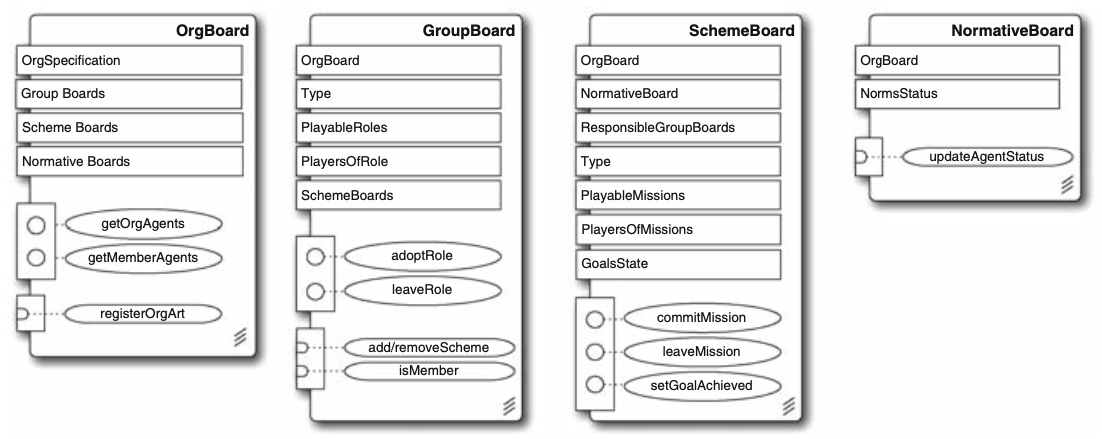
\includegraphics[width=\linewidth]{images/org-artifacts.png}
    \caption{Organizational artifacts in \oraformas{} with their interface including operations, observable properties, and link interfaces. Adopted from~\cite{hubner2010}.}
    \label{fig:org-artifacts}
\end{figure}

\subsubsection{\oraformas{} in Action}
When a set of agents wants to coordinate their actions to achieve a common goal, they can do it, for instance, through the following steps:
\begin{enumerate}
    \item One of the agents, which is also an \textit{organizational agent}, creates an \textsf{OrgBoard} artifact based on a specification.
    \item The organizational agent creates a \textsf{GroupBoard} artifact for each group of agents that will be part of the organization.
    Once the \textsf{GroupBoard} is created,  the artifact registers itself in the \textsf{OrgBoard} exploiting the latter's link interface.
    \item All the other agents get notified about the new artifacts and therefore may decide to adopt a role in one of the groups.
    They can do so using the \textsf{adoptRole} operation of the \textsf{GroupBoard} artifact.
    \item The organizational agent can now create a \textsf{SchemeBoard} artifact to start the organization's collective goals.
    As for the \textsf{GroupBoard}, the \textsf{SchemeBoard} artifact registers itself in the \textsf{OrgBoard}.
    As every \textsf{SchemeBoard} has one \textsf{NormativeBoard}, the latter is created automatically and linked to the former.
    \item Once the \textsf{SchemeBoard} is created, obligations and permissions are computed and verified by the \textsf{NormativeBoard}.
    Agents can now commit to their missions according to the \textsf{NormativeBoard} rules.
    \item Once the scheme is well formed, the goals of the scheme can be achieved by the agents.
\end{enumerate}

\section{Hypermedia Multi-Agent Systems}
The current technological landscape brings new challenges to the engineering of MAS such as the support of large-scale open systems, and the support of heterogeneous agents and humans in the loop.

\subsection{The World Wide Web}
The Web has had remarkable success as a worldwide and long-lived system of people, providing them with a \textit{distributed hypermedia environment}, composed of interrelated Web pages, that they can navigate and use in pursuit of their goals.

No doubt REST (REpresentational State Transfer), the architectural style of the Web~\cite{fielding2000}, is one of the enabling factors of the above characteristics.
REST consists of a set of architectural constraints, such as \textit{client-server} and \textit{stateless} interaction, \textit{uniform interface}.
% Since the World Wide Web (WWW) is claimed to be one of the most successful middleware for the development of distributed systems, and with the recent focus on hypermedia-driven APIs and the Web of Things and Linked Data initiatives, it can be used as a basis for the engineering of MAS.

\subsection{Web-based Multi-Agent Systems}

% Early Web-based MAS
% Why they were not successful
% Hypermedia MAS